\begin{frame}
\frametitle{Атомарный Read/Write регистр}
\begin{itemize}
    \item<1->Атомарный RW регистр - ячейка памяти и пара операций
    \begin{itemize}
        \item<2->write - "атомарно" записывает значение в регистр;
        \item<3->read - "атомарно" читает последнее записанное значение;
        \item<4->все операции (read/write) упорядочены.
    \end{itemize}
\end{itemize}
\end{frame}

\begin{frame}
\frametitle{Взаимное исключение для 2-х потоков}
\begin{itemize}
    \item<1->Есть всего два потока
    \begin{itemize}
        \item<2->потоки имеют идентификаторы 0 и 1;
        \item<3->внутри потока мы можем узнать его идентификатор (пусть за
             это отвечает функция \lstinline|threadId|).
    \end{itemize}
\end{itemize}
\end{frame}

\begin{frame}[fragile]
\frametitle{Альтернация}
\begin{lstlisting}
    struct lock {
        atomic_int last;
    };

    void lock_init(struct lock *lock)
    {
        atomic_store(&lock->last, 0);
    }

    void lock(struct lock *lock)
    {
        while (atomic_load(&lock->last) == threadId());
    }

    void unlock(struct lock *lock)
    {
        atomic_store(&lock->last, threadId());
    }
\end{lstlisting}
\end{frame}

\begin{frame}
\frametitle{Свойство взаимного исключения}
\begin{itemize}
    \item<1->Для приведенного алгоритма взаимное исключение гарантируется
    \begin{itemize}
        \item<2->lock может вернуть управление только потоку с
             идентификатором не равным \lstinline|lock->last|;
        \item<3->только поток с \lstinline|threadId() != lock->last| может
             изменить значение \lstinline|lock->last|.
    \end{itemize}
\end{itemize}
\end{frame}

\begin{frame}
\frametitle{Свойство живости}
\begin{itemize}
    \item<1->Пусть поток 1 вообще никогда не пытается захватить лок
    \begin{itemize}
        \item<2->если поток 0 вызовет lock, то он зависнет навсегда;
        \item<3->т. е. свойство живости не выполняется.
    \end{itemize}
\end{itemize}
\end{frame}

\begin{frame}[fragile]
\frametitle{Флаги намерения}
\begin{lstlisting}
    struct lock {
        atomic_int flag[2];
    };

    void lock_init(struct lock *lock)
    {
        atomic_store(&lock->flag[0], 0);
        atomic_store(&lock->flag[1], 0);
    }

    void lock(struct lock *lock)
    {
        const int me = threadId();
        const int other = 1 - me;

        atomic_store(&lock->flag[me], 1);
        while (atomic_load(&lock->flag[other]));
    }

    void unlock(struct lock *lock)
    {
        const int me = threadId();

        atomic_store(&lock->flag[me], 0);
    }
\end{lstlisting}
\end{frame}

\begin{frame}
\frametitle{Корректность}
\begin{itemize}
    \item<1->Гарантируется ли взаимное исключение?
    \item<2->Гарантируется ли живость?
\end{itemize}
\end{frame}

\begin{frame}[fragile]
\frametitle{Алгоритм Петерсона для 2-х потоков}
\begin{lstlisting}
    struct lock {
        atomic_int last;
        atomic_int flag[2];
    };

    void lock(struct lock *lock)
    {
        const int me = threadId();
        const int other = 1 - me;

        atomic_store(&lock->flag[me], 1);
        atomic_store(&lock->last, me);

        while (atomic_load(lock->flag[other])
               && atomic_load(&lock->last) == me);
    }

    void unlock(struct lock *lock)
    {
        const int me = threadId();

        atomic_store(&lock->flag[me], 0);
    }
\end{lstlisting}
\end{frame}

\begin{frame}
\frametitle{Взаимное исключение}
\begin{itemize}
    \item<1->Доказательство от противного - пусть два потока одновременно
         находятся в критической секции
    \begin{itemize}
        \item<2->оба потока записывали значение в атомарный регистр last;
        \item<3->один из них должен был быть первым, а другой последним;
        \item<4->для определенности, пусть последним был поток 1.
    \end{itemize}
\end{itemize}
\end{frame}

\begin{frame}
\frametitle{Взаимное исключение}
\begin{itemize}
    \item<1->Итак нам известно следующее:
    \begin{itemize}
        \item<2->\lstinline|lock->last == 1| - последним туда записал поток 1;
        \item<3->\lstinline|lock->flag[0] = 1| и \lstinline|lock->flag[1] == 1|.
    \end{itemize}
\end{itemize}
\end{frame}

\begin{frame}
\frametitle{Взаимное исключение}
\begin{itemize}
    \item<1->Как в таких условиях поток 1 мог пройти мимо цикла в lock и войти
         в критическую секцию?
    \begin{itemize}
        \item<2->очевидно, никак.
    \end{itemize}
\end{itemize}
\end{frame}

\begin{frame}
\frametitle{Живость}
\begin{itemize}
     \item<1->Пусть поток 0 пытается войти в критическую секцию, возможны две
          ситуации:
     \begin{itemize}
         \item<2->при проверке условия цикла \lstinline|lock->flag[1] == 0|;
         \item<3->при проверке условия цикла \lstinline|lock->flag[1] == 1|.
     \end{itemize}
\end{itemize}
\end{frame}

\begin{frame}
\frametitle{Живость}
\begin{itemize}
    \item<1->В первом случае (\lstinline|lock->flag[1] == 0|)
    \begin{itemize}
        \item<2->поток 1 даже не пытался захватить блокировку;
        \item<3->условие цикла, очевидно, ложно, и поток 0 входит в
             критическую секцию
    \end{itemize}
\end{itemize}
\end{frame}

\begin{frame}
\frametitle{Живость}
\begin{itemize}
    \item<1->Во втором случае (\lstinline|lock->flag[1] == 1|)
    \begin{itemize}
        \item<2->оба потока изъявили намерение войти в критическую секцию;
        \item<3->нужно показать, что хотя бы один из них рано или поздно
             зайдет в критическую секцию (или уже зашел).
    \end{itemize}
\end{itemize}
\end{frame}

\begin{frame}
\frametitle{Живость}
\begin{itemize}
    \item<1->Оба потока, после записи в \lstinline|lock->flag[x]| должны, в
         какой-то момент, записать в \lstinline|lock->last|
    \begin{itemize}
        \item<2->не трудно увидеть, что если \lstinline|lock->flag[0] == 1| и
             \lstinline|lock->flag[1] == 1|,
        \item<2->то тот из них, кто сделал это первым войдет в критическую
             секцию.
    \end{itemize}
\end{itemize}
\end{frame}


\begin{frame}
\frametitle{N потоков}
\begin{itemize}
    \item<1->Реализовав взаимное исключение для 2-х потоков мы можем
         реализовать вазимное исключение для любого числа потоков
    \begin{itemize}
        \item<2->организуем турнир для N потоков;
        \item<3->потоки конкурируют друг с другом на "выбывание".
    \end{itemize}
\end{itemize}
\end{frame}

\begin{frame}
\frametitle{N потоков}
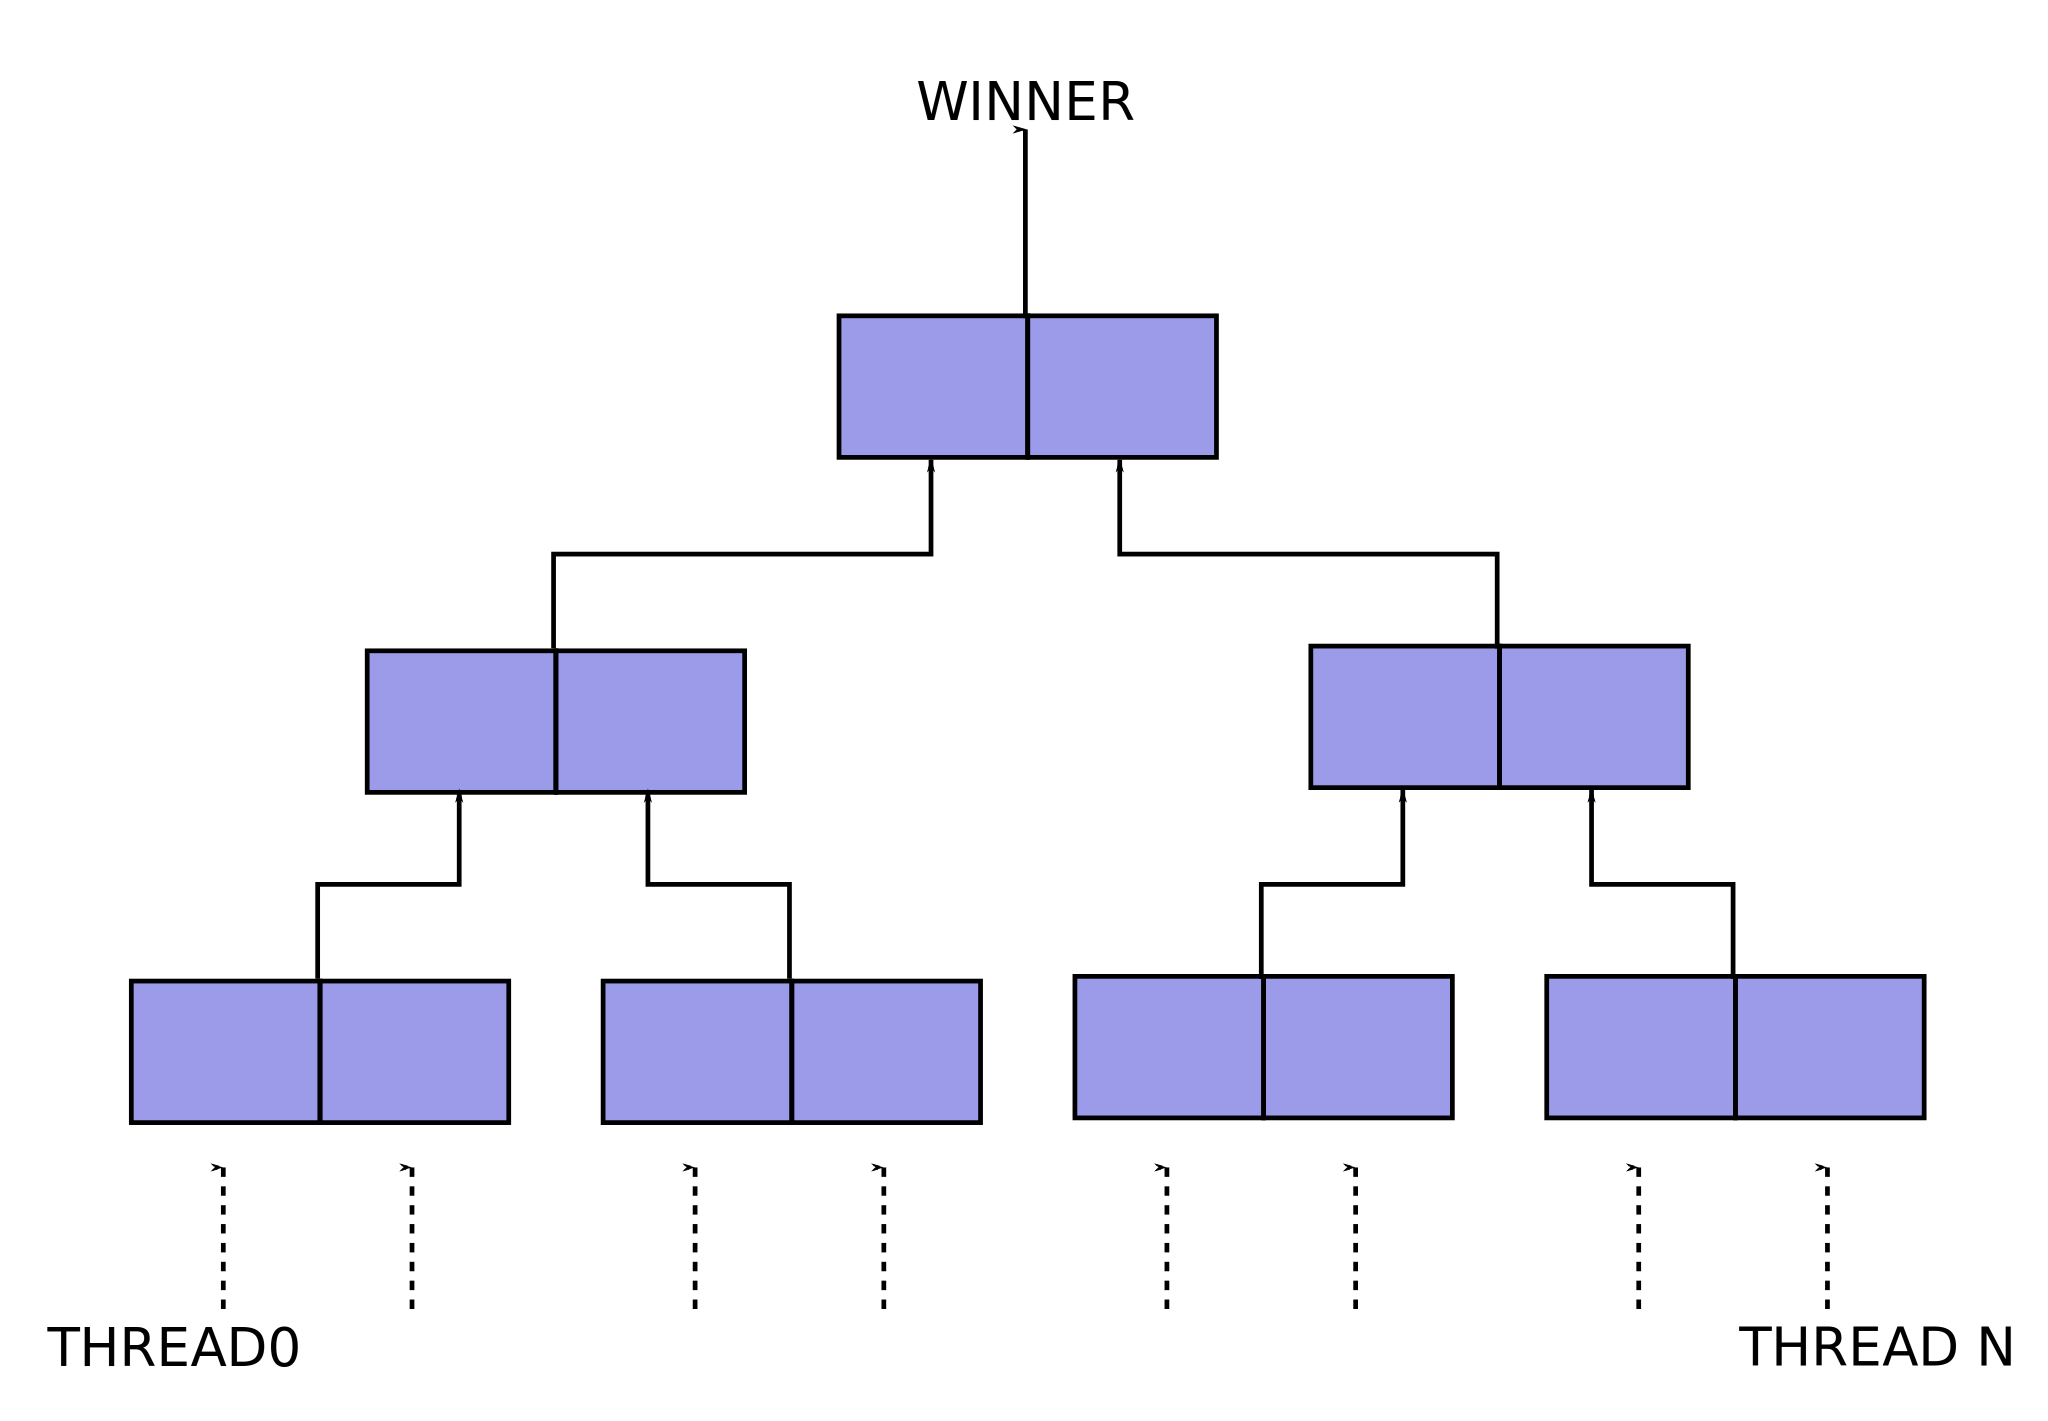
\includegraphics[height=.5\textheight]{nthreads}
\end{frame}

\begin{frame}[fragile]
\frametitle{Алгоритм Петерсона для N потоков}
\begin{lstlisting}
    struct lock_one {
        atomic_int last;
        atomic_int flag[N];
    };

    int flags_clear(const struct lock_one *lock)
    {
        const int me = threadId();

        for (int i = 0; i != N; ++i) {
            if (i != me && atomic_load(&lock->flag[i]))
                return 0;
        }
        return 1;
    }

    void lock_one(struct lock_one *lock)
    {
        const int me = threadId();

        atomic_store(&lock->flag[me], 1);
        atomic_store(&lock->last, me);

        while (!flags_clear(lock)
               && atomic_load(&lock->last) == me);
    }

    void unlock_one(struct lock_one *lock)
    {
        const int me = threadId();

        atomic_store(&lock->flag[me], 0);
    }
\end{lstlisting}
\end{frame}

\begin{frame}[fragile]
\frametitle{Алгоритм Петерсона для N потоков}
\begin{lstlisting}
    struct lock {
        struct lock_one lock[N - 1];
    };

    void lock(struct lock *lock)
    {
        for (int i = 0; i != N - 1; ++i)
            lock_one(&lock->lock[i]);
    }

    void unlock(struct lock *lock)
    {
        for (int i = N - 2; i >= 0; --i)
            unlock_one(&lock->lock[i]);
    }
\end{lstlisting}
\end{frame}

\begin{frame}[fragile]
\frametitle{Алгоритм Петерсона для N потоков}
\begin{lstlisting}
    struct lock {
        atomic_int level[N];
        atomic_int last[N - 1];
    };

    void lock(struct lock *lock)
    {
        const int me = threadId();

        for (int i = 0; i != N - 1; ++i) {
            atomic_store(&lock->level[me], i + 1);
            atomic_store(&lock->last[i], me);

            while (!flags_clear(lock, i)
                   && atomic_load(&lock->last[i]) == me);
        }
    }

    void unlock(struct lock *lock)
    {
        const int me = threadId();

        atomic_store(&lock->level[me], 0);
    }
\end{lstlisting}
\end{frame}

\begin{frame}
\frametitle{Честность}
\begin{itemize}
    \item<1->Не хочется, чтобы потоки голодали!
    \begin{itemize}
        \item<2->если поток захотел захватить блокировку, то когда-нибудь
             ему это удастся;
        \item<3->сравните с живостью - среди потоков, пытающихся захватить
             блокировку, одному это удастся.
    \end{itemize}
\end{itemize}
\end{frame}

\begin{frame}
\frametitle{Супер честность}
\begin{itemize}
    \item<1->k-ограниченное ожидание:
    \begin{itemize}
        \item<2->после того как поток "изяъвил" желание захватить блокировку
             (встал в очередь), не более k потоков могут пролезть вперед него
             без очереди.
    \end{itemize}
\end{itemize}
\end{frame}

\begin{frame}
\frametitle{Алгоритм Петерсона на примере 3 потоков}
\begin{table}
\begin{tabular}{l | c | c | c | c | c }
№ & level[0] & level[1] & level[2] & last[0] & last[1] \\
\hline\hline

0 & 0 & 0 & 0 & 0 & 0 \\
1 & 1 & 0 & 0 & 0 & 0 \\
2 & 1 & 1 & 0 & 1 & 0 \\
3 & 1 & 1 & 1 & 2 & 0 \\
4 & 2 & 1 & 1 & 2 & 0 \\
5 & 0 & 1 & 1 & 2 & 0 \\
6 & 1 & 1 & 1 & 0 & 0 \\
7 & 1 & 1 & 2 & 0 & 2 \\
8 & 1 & 1 & 0 & 0 & 2 \\
9 & 1 & 1 & 1 & 2 & 2 \\
10 & 2 & 1 & 1 & 2 & 0 \\

\hline
\end{tabular}
\end{table}
\end{frame}
